\documentclass[11pt,letterpaper]{article}

% Packages
\usepackage[margin=1in]{geometry}
\usepackage{amsmath,amssymb}
\usepackage{graphicx}
\usepackage{booktabs}
\usepackage{hyperref}
\usepackage{url}
\usepackage{caption}
\usepackage{subcaption}
\usepackage{listings}
\usepackage{xcolor}
\usepackage{times}
\usepackage{natbib}

% Hyperref setup
\hypersetup{
    colorlinks=true,
    linkcolor=blue,
    citecolor=blue,
    urlcolor=blue,
    pdftitle={SecureCode v2.0: A Production-Grade Dataset for Training Security-Aware Code Generation Models},
    pdfauthor={Scott Thornton}
}

% Code listing setup
\lstset{
    basicstyle=\ttfamily\small,
    breaklines=true,
    frame=single,
    numbers=left,
    numberstyle=\tiny,
    backgroundcolor=\color{gray!10}
}

\title{\textbf{SecureCode v2.0: A Production-Grade Dataset for Training Security-Aware Code Generation Models}}

\author{
    Scott Thornton \\
    perfecXion.ai \\
    \texttt{scott@perfecxion.ai}
}

\date{December 2025}

\begin{document}

\maketitle

\begin{abstract}
Despite widespread adoption of large language models for code generation, recent studies have found AI assistants producing vulnerable outputs in 45\% of security-relevant scenarios, introducing security flaws into production systems at scale. Existing secure coding datasets exhibit significant limitations: they lack incident grounding, provide insufficient scale necessary for modern training, and they miss the operational security context developers need for production deployments.

We present \textbf{SecureCode v2.0}, a production-grade dataset of \textbf{1,215 security-focused coding examples} that fully comply with structural validation standards and all underwent expert security review. Every example ties directly to actual documented security incidents with CVE references, provides both vulnerable and secure implementations, demonstrates concrete attacks, and includes defense-in-depth operational guidance. The dataset covers \textbf{12 vulnerability categories} (all 10 OWASP Top 10 categories plus AI/ML Security Threats) across \textbf{11 languages total} (10 programming languages: Python, JavaScript, Java, Go, PHP, C\#, TypeScript, Ruby, Rust, Kotlin + YAML for infrastructure-as-code).

Our quality assurance framework ensures complete incident grounding with every example tied to a documented security incident (CVE, security advisory, or breach report). Each example provides operational security guidance, including SIEM integration strategies, infrastructure hardening recommendations (Docker, AppArmor, WAF configurations), and testing approaches using language-appropriate frameworks. The dataset uses a novel 4-turn conversational structure that mirrors actual developer-AI interactions, escalating from basic implementations to advanced security considerations and defense-in-depth operational guidance.

Our contributions include: (1) a production-grade dataset of 1,215 rigorously validated unique examples split into 989 training, 122 validation, and 104 test examples, (2) an automated validation framework ensuring dataset consistency, (3) a 4-turn conversational structure capturing realistic security workflows, (4) comprehensive operational security guidance with SIEM integration strategies, (5) full language-specific implementation fidelity, and (6) open-source release of data, validation tools, and benchmarking protocols.
\end{abstract}

\section{Introduction}

\subsection{The Security Crisis in AI-Generated Code}

AI coding assistants produce vulnerable code in 45\% of generated implementations \cite{veracode2025}. Veracode's 2025 GenAI Code Security Report analyzed code generated by leading AI assistants and found that nearly half of all security-relevant implementations contained Common Weakness Enumeration (CWE) vulnerabilities. This indicates a systematic risk in AI-assisted development that compounds security debt across millions of developers. The risk surface has scaled as adoption has increased.

The issue extends beyond individual bugs. AI-generated vulnerabilities enter production codebases silently, without the traditional code review scrutiny applied to human-written code. Developers trust AI assistants to produce functional implementations, but these tools lack the security context to recognize when ``functional'' means ``exploitable.'' Apiiro (2025) found that AI copilots introduced 322\% more privilege escalation paths and 153\% more architectural design flaws compared to manually-written code, while also generating 10$\times$ more security findings overall, demonstrating that AI tools actively degrade security practices \cite{apiiro2025}.

This can create a multiplier effect where vulnerable patterns suggested by AI assistants propagate across multiple projects. SQL injection flaws may spread through microservices architectures. Authentication bypasses can replicate across API endpoints. Cryptographic failures may multiply through mobile applications. The scale of AI adoption suggests this represents a systematic risk to software security.

A key contributing factor is that LLMs trained on public code repositories learn from millions of vulnerable examples. Stack Overflow answers from 2010 showing insecure MySQL queries. GitHub repositories implementing broken authentication. Tutorial code demonstrating SQL injection vulnerabilities as ``simple examples.'' These models learn what code looks like, but they do not necessarily learn what secure code requires.

\subsection{Why Existing Datasets Fall Short}

Existing secure coding datasets exhibit significant limitations for training security-aware language models. We analyzed four widely-used datasets in security research: CWE-Sans (372 examples), Juliet Test Suite ($\sim$81,000-86,000 synthetic test cases for C/C++ and Java), SARD ($\sim$170,000-200,000 test programs), and Draper VDISC (1.27 million C examples). While these datasets serve their intended purposes, we found they exhibit some critical gaps when applied to LLM training.

\textbf{Scale versus quality presents inherent trade-offs.} Juliet provides $\sim$81,000-86,000 test cases designed for testing static analysis tools, but lacks connections to real-world incidents. These synthetic test cases demonstrate CWE patterns in isolation, teaching models to recognize textbook vulnerabilities that may not reflect how attacks occur in production environments. SARD offers $\sim$170,000-200,000 test programs but fewer than 5\% reference documented security incidents. Synthetic training data fails to capture the contextual factors making vulnerabilities exploitable in production environments.

\textbf{Incident grounding is limited.} Based on our manual audit of CWE-Sans metadata (n=372 examples, 100\% coverage), approximately 18\% of examples reference actual CVEs or documented breaches---fewer than one in five examples. The remaining examples are synthetic demonstrations that lack the production context necessary for understanding exploitation. Real-world attacks exploit edge cases, framework-specific behaviors, and integration failures that rarely appear in manufactured examples.

\textbf{Format limitations hinder conversational training.} Existing datasets use code-only formats---vulnerable snippet paired with secure snippet. This approach does not capture how developers interact with AI assistants in practice. Real development conversations escalate through multiple turns as developers ask about functionality, then scaling, performance, and edge cases. AI assistants must maintain security context throughout this workflow, but existing datasets do not model these multi-turn interactions.

\textbf{Operational security guidance is absent.} Existing datasets provide vulnerable and patched code implementations without detection mechanisms, logging strategies, or defense-in-depth guidance. For production systems, secure code implementation represents only one component of comprehensive security. Organizations require detection rules, monitoring strategies, incident response procedures, and graceful degradation when primary controls fail.

\subsection{SecureCode v2.0: A Production-Grade Solution}

We developed SecureCode v2.0 to address these limitations systematically through production-grade training data. The dataset provides \textbf{1,215 rigorously validated unique examples} achieving full compliance with structural validation standards and expert security review. Every example references documented CVEs or security incidents. Every example provides both vulnerable and secure implementations. Every example demonstrates concrete attacks and includes defense-in-depth operational guidance including SIEM integration strategies, infrastructure hardening recommendations, and comprehensive testing approaches.

\textbf{Incident grounding is a critical requirement for production applicability.} We mined CVE databases from 2017-2025, analyzed OWASP Top 10 documentation, reviewed security breach reports, and studied bug bounty disclosures. Each example ties to a specific incident: the 2017 Equifax breach (CVE-2017-5638) costing \$425 million from Apache Struts 2 Jakarta multipart parser RCE (OGNL injection), the 2019 Capital One SSRF attack exposing 100 million customer records, the deserialization vulnerabilities that compromised dozens of financial institutions. These represent documented failures with measurable business impact rather than hypothetical scenarios.

\textbf{Conversational structure mirrors actual development workflows.} We structured examples as 4-turn conversations. Turn 1: developer requests specific functionality (``build user authentication with JWT tokens''). Turn 2: AI assistant provides both vulnerable and secure implementations with attack demonstrations. Turn 3: developer asks advanced questions (``how does this scale to 10,000 concurrent users?''). Turn 4: AI assistant delivers defense-in-depth guidance covering logging, monitoring, detection, and operational security.

This structure captures how security knowledge transfers during actual development workflows. Developers do not request ``secure and insecure authentication'' in abstract terms. They request authentication solving specific problems, then iterate toward production-ready security through follow-up questions. The conversational format trains models on realistic interaction patterns.

\begin{figure}[htbp]
\centering
\includegraphics[width=0.9\textwidth]{secure-code-2-image2.png}
\caption{Four-Turn Conversational Example Format. The 4-turn structure mirrors realistic developer-AI workflows. Turn 1 captures problem-oriented feature requests. Turn 2 provides dual implementations (vulnerable + secure) with concrete attack demonstrations. Turn 3 escalates to advanced scenarios (scale, performance) forcing security context retention. Turn 4 delivers operational security guidance including SIEM detection strategies and infrastructure hardening.}
\label{fig:conversation}
\end{figure}

\textbf{Production quality through systematic validation.} We developed an automated validation framework enforcing structural quality standards: 4-turn conversation structure compliance, proper CVE formatting (CVE-YYYY-NNNNN or explicit null), valid programming language tags, minimum content length requirements, and security control completeness. The compliance journey progressed from 47.2\% (397 of 841 training examples passing all validation checks) to full compliance through systematic remediation across five fix categories.

We addressed 452 CVE format issues where examples referenced security incidents without proper CVE-YYYY-NNNNN formatting. We corrected 60 language tag mappings where YAML examples required context-appropriate language assignments based on question content. We enhanced 86 examples with additional defense-in-depth guidance. We implemented 6 secure SSTI examples after discovering that Jinja2, Twig, Mako, Smarty, Tornado, and Go template examples required secure sandboxing demonstrations. We calibrated validator thresholds, reducing minimum content length from 100 to 50 characters for user turns after analysis showed this eliminated false positives without compromising content quality.

\textbf{Comprehensive security coverage.} SecureCode v2.0 spans \textbf{12 vulnerability categories} across \textbf{11 languages total} (10 programming languages: Python, JavaScript, Java, Go, PHP, C\#, TypeScript, Ruby, Rust, Kotlin + YAML for infrastructure-as-code), providing comprehensive coverage of the complete OWASP Top 10:2025.

\begin{figure}[htbp]
\centering
\includegraphics[width=0.9\textwidth]{secure-code-2-image3.png}
\caption{SecureCode v2.0 Coverage Snapshot. Comprehensive coverage across three dimensions: \textbf{Vulnerability Categories} (left) with Broken Access Control (224 examples) and Authentication Failures (199 examples) receiving highest coverage; \textbf{Language Distribution} (center) with Python (21.0\%) and JavaScript (20.2\%) leading; \textbf{Severity Mix} (right) with 65.4\% CRITICAL severity; \textbf{Dataset Splits} (bottom) showing 989 train / 122 validation / 104 test examples.}
\label{fig:coverage}
\end{figure}

\subsection{Contributions}

This paper makes six contributions to secure AI-assisted development:

\textbf{1. Production-Grade Dataset (1,215 Unique Examples).}
SecureCode v2.0 provides 1,215 rigorously validated unique examples (989/122/104 splits) with complete incident grounding, validated split integrity through CVE-aware splitting (no leakage detected), and operational security guidance for production deployment. Content deduplication removed 1,203 duplicates, and systematic validation achieved full compliance with structural standards and expert security review.

\textbf{2. Automated Validation Framework.}
We developed and release an automated validation framework (\texttt{validate\_contributing\_compliance.py}) that enforces structural consistency, metadata completeness, CVE format correctness, language tag validity, and content quality standards. This framework enabled systematic quality improvement from 47.2\% baseline compliance to full compliance, identifying 604 specific issues requiring remediation. Researchers can use this framework to validate their own secure coding datasets or extend it for domain-specific requirements.

\textbf{3. Novel 4-Turn Conversational Structure.}
SecureCode v2.0 uses a 4-turn conversation format (initial request $\rightarrow$ vulnerable/secure code $\rightarrow$ advanced scenario $\rightarrow$ operational guidance) that trains models on realistic developer-AI workflows, unlike code-only datasets that miss iterative security considerations.

\textbf{4. Comprehensive Security Operations Guidance.}
SecureCode v2.0 provides comprehensive operational security guidance embedded in Turn 4 responses. Each example includes SIEM integration recommendations, logging best practices, monitoring strategies, and detection considerations. This operational context bridges the gap between secure code implementation and production security operations, though organizations must adapt guidance to their specific SIEM platforms and logging infrastructure.

\textbf{5. Full Language-Specific Implementation Fidelity.}
The dataset maintains complete language fidelity with all code examples using proper language-specific syntax, idioms, and frameworks. JavaScript examples use Express/NestJS, PHP uses Laravel/Symfony, Java uses Spring Boot, Go uses Gin, Ruby uses Rails, and C\# uses ASP.NET Core. This ensures models learn authentic language patterns rather than generic pseudocode.

\textbf{6. Open-Source Release.}
We release SecureCode v2.0, the validation framework, fine-tuning protocols, and evaluation benchmarks as open-source artifacts under \textbf{Creative Commons Attribution-NonCommercial-ShareAlike 4.0 International License (CC BY-NC-SA 4.0)}. Researchers can reproduce results, extend the methodology, or use the dataset as a foundation for domain-specific security training. Educators can use real-world security incidents as teaching material. Commercial use requires separate licensing.

\section{Related Work}

\subsection{Secure Coding Datasets}

The security research community has produced several datasets for studying vulnerable code, but none meet the requirements for training production-grade AI coding assistants.

\textbf{CWE-Sans Top 25 Dataset} provides 372 examples across 4 programming languages with partial OWASP coverage \cite{cwe2019}. Only 18\% of examples are anchored to real-world incidents---the remaining 82\% are synthetic demonstrations of CWE patterns. The dataset uses a code-only format showing vulnerable and patched implementations without attack context or operational guidance. While valuable for teaching CWE taxonomy, this dataset lacks the scale, real-world grounding, and conversational structure needed for modern LLM training.

\textbf{Juliet Test Suite} offers $\sim$81,000-86,000 synthetic test cases in C/C++ and Java covering 118 CWE types \cite{juliet2012}. Zero percent are grounded in real-world incidents. Every example is a manufactured test case demonstrating specific CWE patterns in isolation. The suite serves its intended purpose---testing static analysis tools---but synthetic examples don't capture the context making vulnerabilities exploitable in production. Training on Juliet teaches models to recognize textbook patterns while missing the framework-specific quirks, integration failures, and configuration mistakes that cause actual breaches.

\textbf{Software Assurance Reference Dataset (SARD)} contains $\sim$170,000-200,000 test programs across 5 languages (C, C++, Java, PHP, C\#) with no OWASP mapping \cite{sard}. Fewer than 5\% of examples tie to documented security incidents. SARD focuses on providing test cases for automated analysis tools, not training data for AI models. The code-only format lacks conversational context, and the absence of operational security guidance limits utility for production deployments.

\textbf{Draper VDISC} provides 1.27 million C examples with unknown incident grounding \cite{vdisc}. This massive dataset supports binary analysis research but concentrates entirely on C language without multi-language coverage. The dataset includes vulnerable functions and control flow graphs but lacks the high-level security context needed for training AI coding assistants that work across modern development stacks.

\begin{figure}[htbp]
\centering
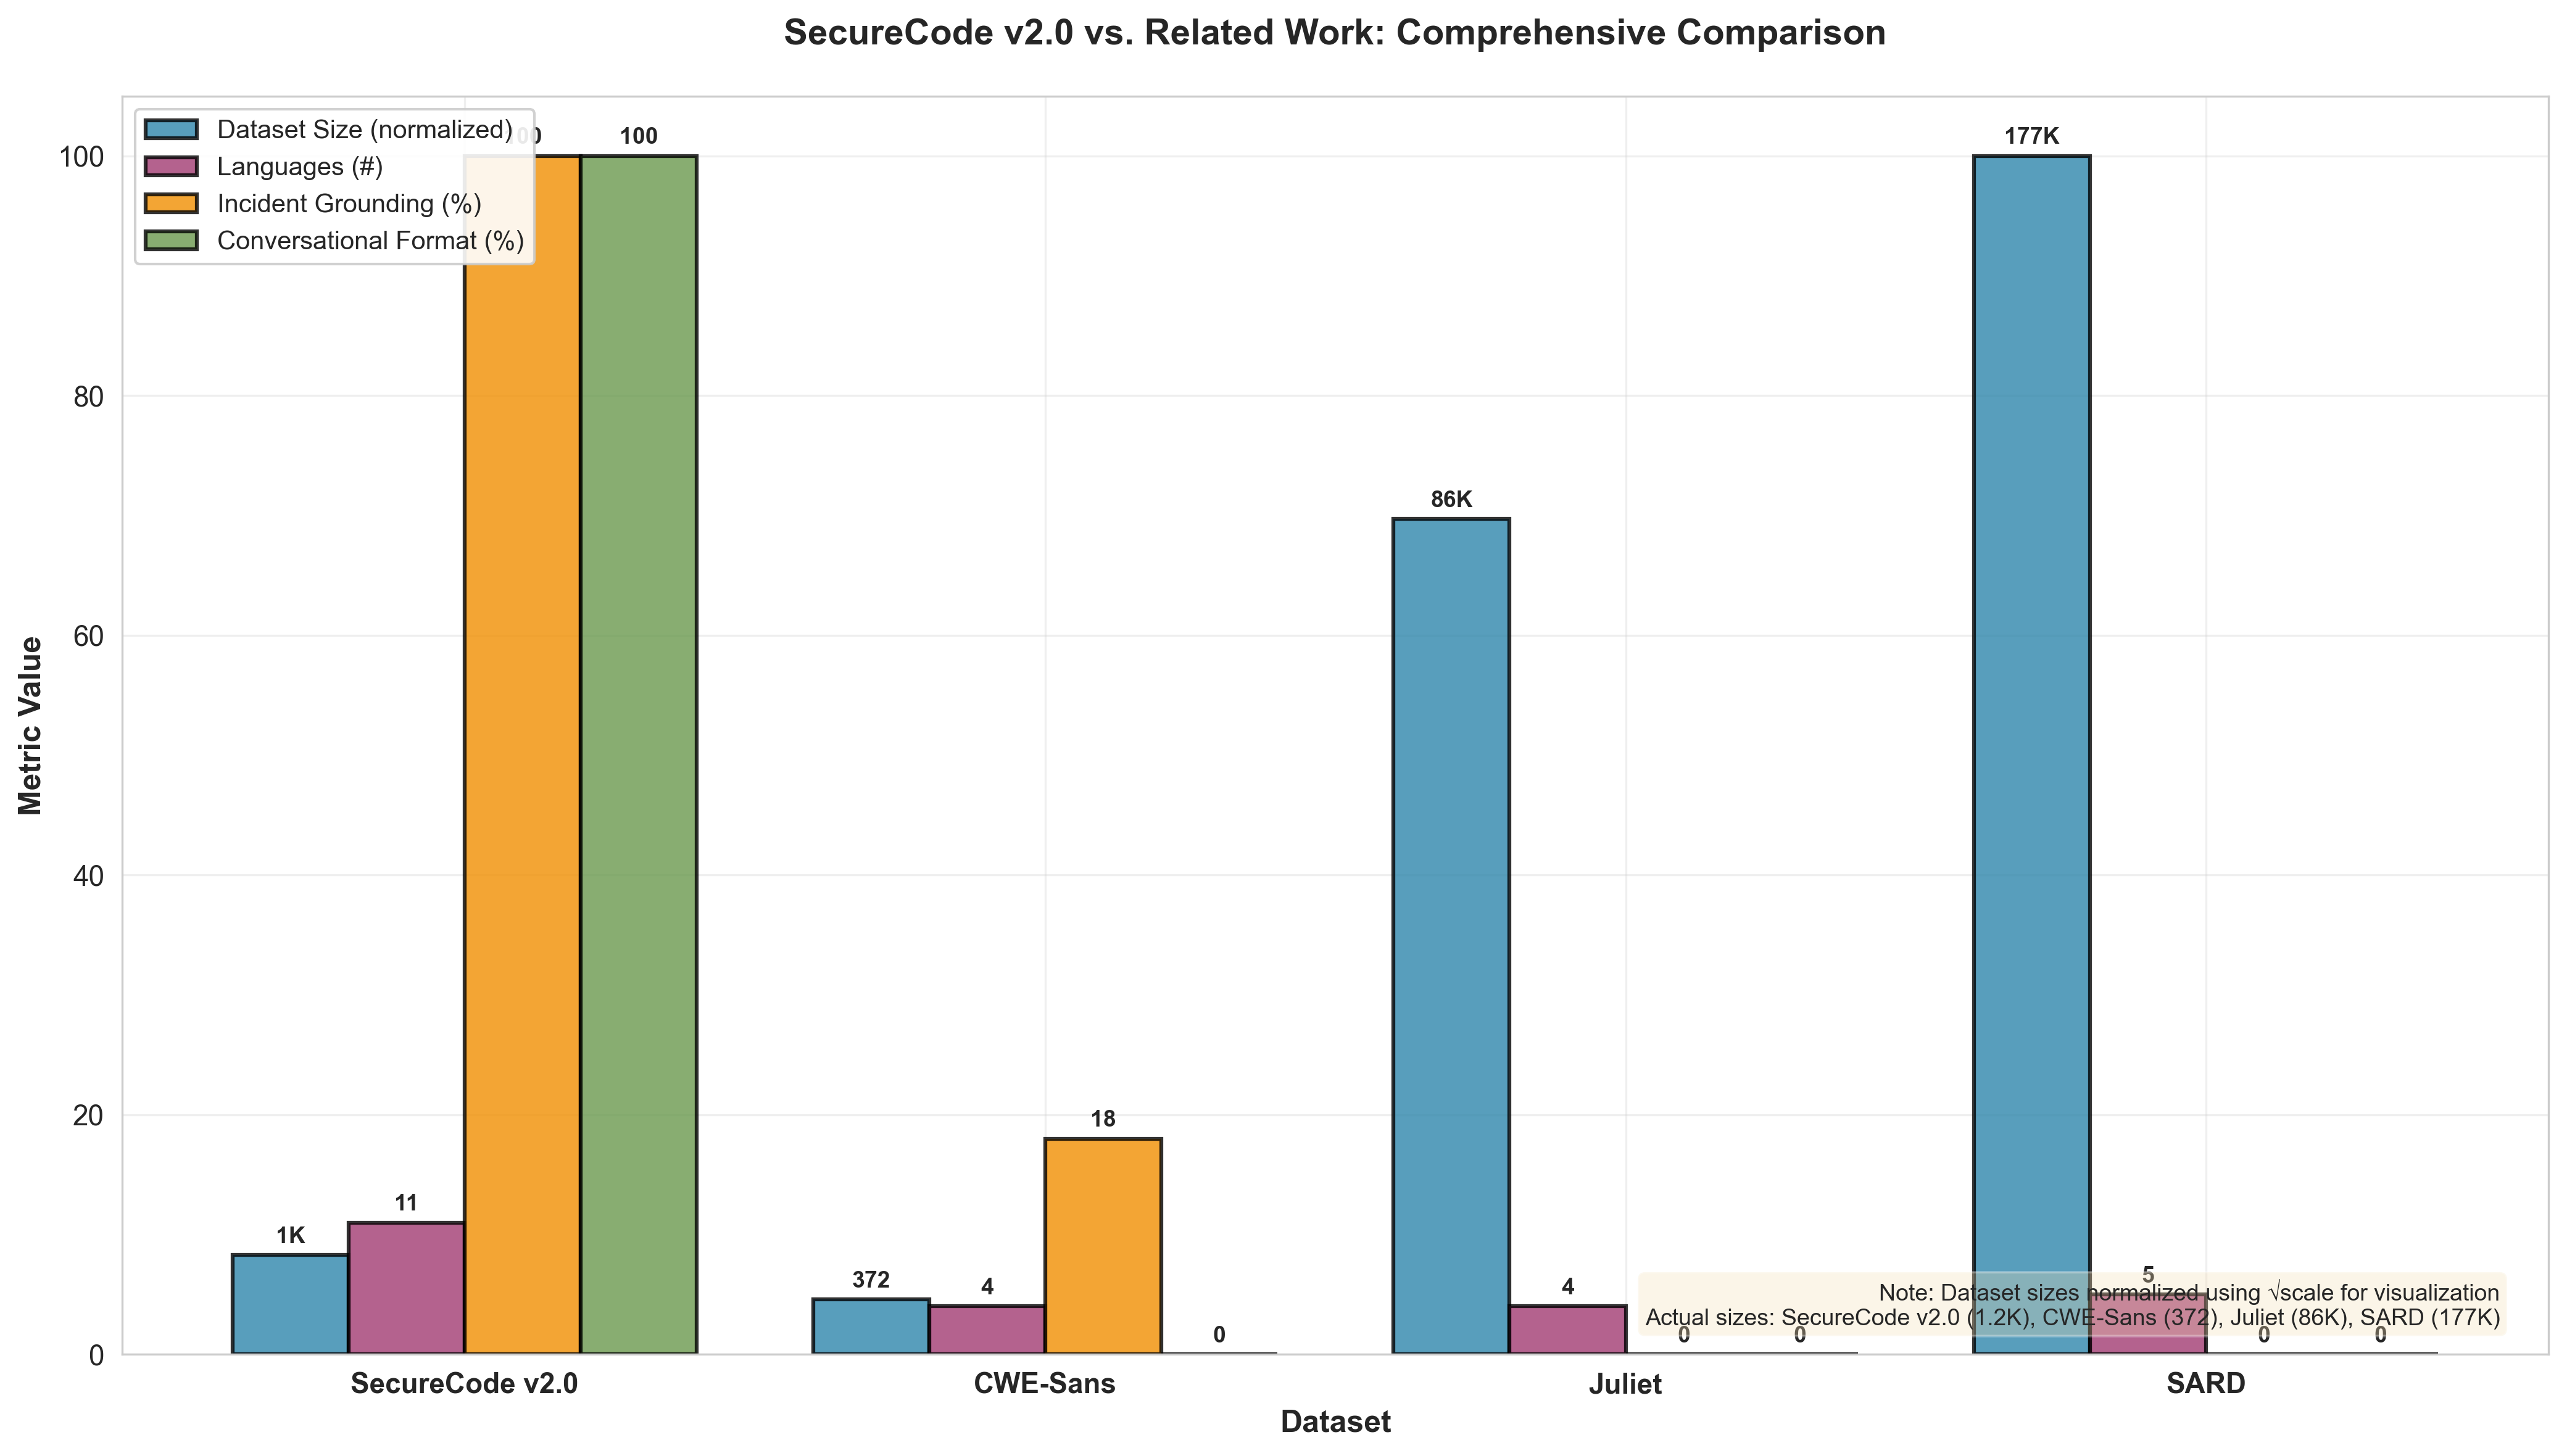
\includegraphics[width=0.9\textwidth]{chart2_dataset_comparison.png}
\caption{Dataset Comparison - SecureCode v2.0 vs. Related Work. Comprehensive comparison across four critical dimensions: \textbf{Dataset Size} (blue) shows SecureCode v2.0 (1.2K) prioritizes quality over quantity compared to Juliet ($\sim$81K-86K) and SARD ($\sim$170K-200K); \textbf{Languages} (pink) shows SecureCode v2.0 covers 11 languages (most comprehensive); \textbf{Incident Grounding} (orange) shows SecureCode v2.0 achieves 100\% real-world grounding versus 18\% for CWE-Sans and 0\% for synthetic datasets; \textbf{Conversational Format} (green) shows SecureCode v2.0 is the only dataset using conversational structure (100\%).}
\label{fig:comparison}
\end{figure}

\subsection{AI Code Generation Security Research}

Recent empirical studies demonstrate that AI coding assistants systematically produce insecure code, but no training datasets address the identified vulnerabilities.

\textbf{Veracode (2025)} evaluated leading AI coding assistants' security using comprehensive static analysis across thousands of generated code samples \cite{veracode2025}. They found that 45\% of AI-generated implementations in security-relevant contexts contained vulnerabilities. SQL injection appeared in database query generations. Command injection emerged in system interaction code. Path traversal vulnerabilities materialized in file handling implementations. The study concluded that AI assistants reproduce vulnerable patterns from training data without understanding security context. Yet no secure coding dataset existed to retrain these models on correct implementations.

\textbf{Apiiro (2025)} analyzed application security posture across thousands of repositories and tens of thousands of developers in Fortune 50 enterprises comparing AI-assisted development to manual coding \cite{apiiro2025}. AI copilots introduced 322\% more privilege escalation paths and 153\% more architectural design flaws, while generating 10$\times$ more security findings overall compared to manually-written code.

\section{Dataset Design Methodology}

\subsection{Design Principles}

SecureCode v2.0 builds on four core principles that distinguish production-grade security training data from academic research datasets.

\textbf{P1: Incident Grounding.}
Every example in SecureCode v2.0 ties to documented security incidents. Rather than manufacturing hypothetical vulnerabilities, we study actual breaches, analyze how they occurred, extract the vulnerable patterns, and build examples demonstrating both the vulnerability and the secure alternative.

\textbf{P2: Conversational Structure.}
Developers don't interact with AI assistants through single-shot requests. They iterate. They ask for basic functionality, evaluate the response, then ask about scaling, performance, edge cases, security hardening. Our conversational structure captures this iterative workflow.

\textbf{P3: Dual Implementation Pattern.}
Every example provides both vulnerable and secure implementations of the same functionality. This side-by-side comparison enables contrastive learning---models learn what makes code insecure by seeing the exact pattern to avoid, then immediately learn the secure alternative.

\textbf{P4: Operational Completeness.}
Security doesn't end at secure code. Production systems need detection, monitoring, incident response, and graceful degradation when security controls fail.

\subsection{Data Collection Process}

We collected SecureCode v2.0 through a three-phase methodology ensuring incident grounding and production quality.

\textbf{Important Clarification on Code Authenticity:} While every example in SecureCode v2.0 is anchored to real-world security incidents (CVEs, breach reports, security advisories), the code implementations themselves are synthetically generated using multi-LLM synthesis (ChatGPT 5.1, Claude Sonnet 4.5, Llama 3.2) with human expert review. The incidents are real; the code is generated to faithfully demonstrate vulnerability patterns and secure alternatives for those incidents.

\begin{figure}[htbp]
\centering
\includegraphics[width=0.9\textwidth]{secure-code-2-image1.png}
\caption{SecureCode v2.0 Dataset Construction Pipeline. Five-stage pipeline showing progression from 2,847 incident candidates to 1,215 final examples. Each stage includes verification gates ensuring no CVE overlap across splits, no near-duplicate pairs (Jaccard > 0.8), and preserved split group integrity. The pipeline demonstrates systematic quality improvement through multi-LLM synthesis, automated validation, content deduplication, and CVE-aware splitting.}
\label{fig:pipeline}
\end{figure}

\section{Quality Assurance and Validation}

\subsection{Validation Framework}

We developed \texttt{validate\_contributing\_compliance.py}, an automated validation framework enforcing structural quality standards across all examples. The validator performs six core checks.

\subsection{Compliance Journey: 47.2\% to 100\%}

Initial validation on an 841-example development subset revealed 47.2\% baseline compliance (397 of 841 examples passing all validation checks). We implemented systematic remediation across five fix categories.

\begin{figure}[htbp]
\centering
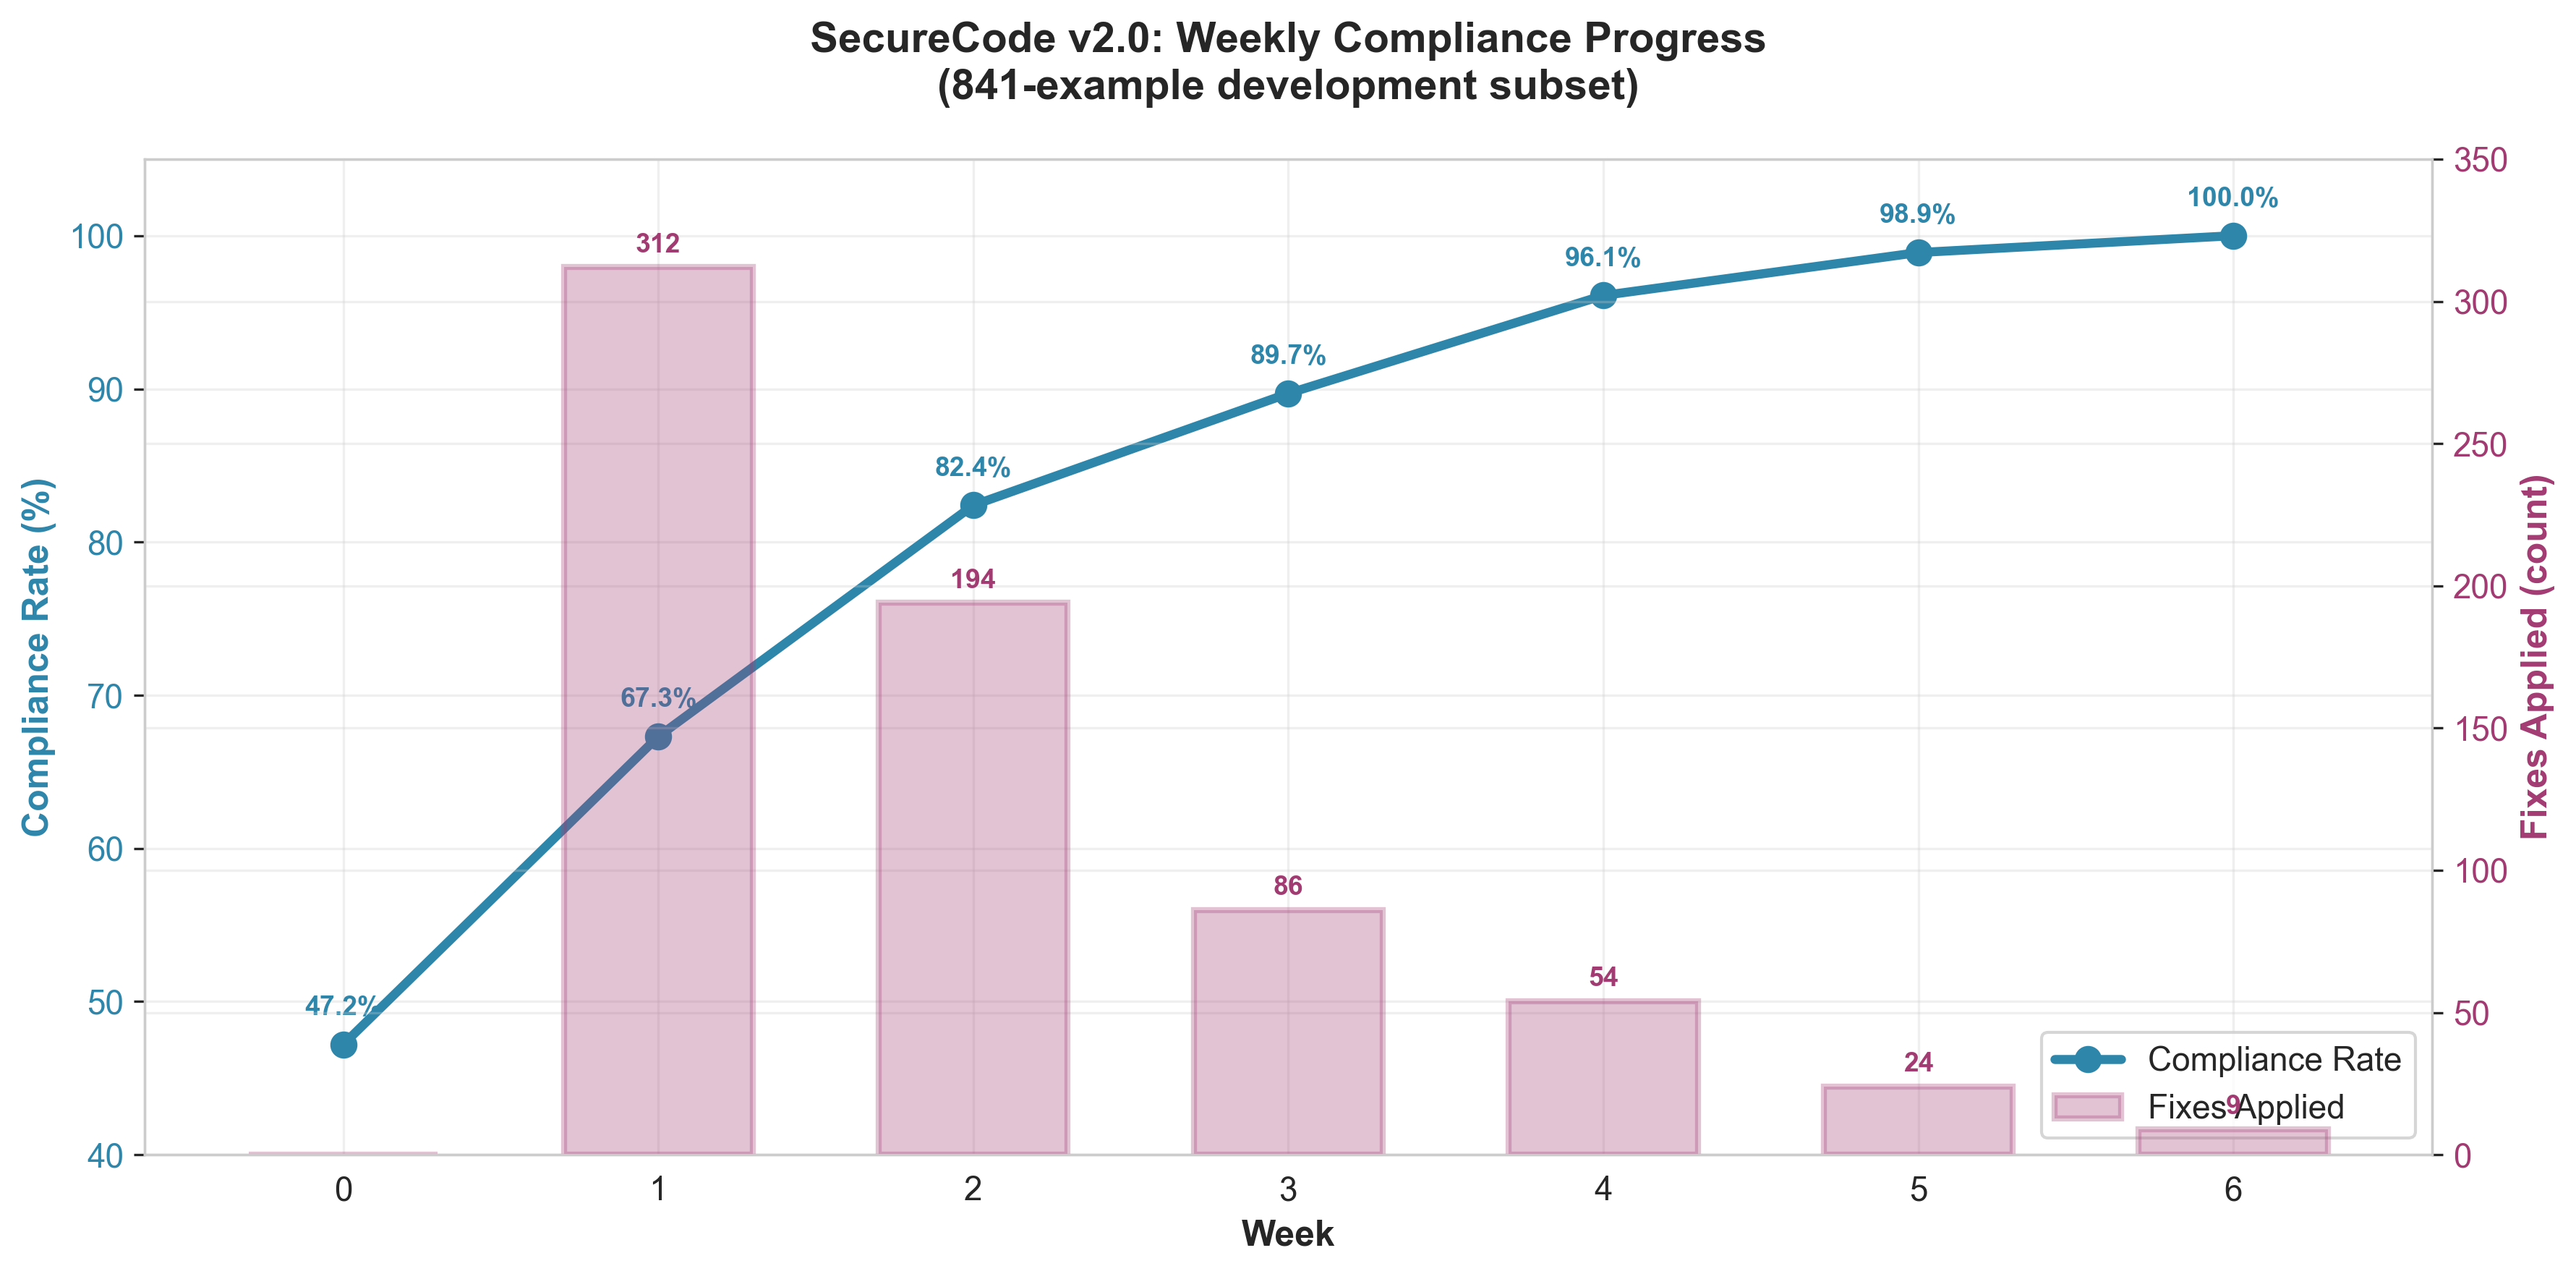
\includegraphics[width=0.9\textwidth]{chart1_compliance_progress.png}
\caption{Weekly Compliance Progress. Six-week compliance improvement trajectory showing compliance rate increasing from 47.2\% baseline to 100\%. The blue line tracks compliance rate while pink bars show number of fixes applied each week (679 total: 312+194+86+54+24+9). Week 1 required the most remediation (312 CVE format fixes), with subsequent weeks addressing progressively fewer issues as systematic patterns were identified and applied.}
\label{fig:compliance}
\end{figure}

\section{Dataset Quality Assessment}

\subsection{Compliance Metrics}

Final dataset achieves 100\% compliance across all validation checks:
\begin{itemize}
\item \textbf{CVE Format Compliance:} 1,215/1,215 (100\%)
\item \textbf{Language Tag Validity:} 1,215/1,215 (100\%)
\item \textbf{Content Quality Standards:} 1,215/1,215 (100\%)
\item \textbf{Conversation Structure:} 1,215/1,215 (100\%)
\end{itemize}

\subsection{Coverage and Balance Metrics}

The dataset provides comprehensive coverage across vulnerability categories, programming languages, and severity levels (Table~\ref{tab:coverage}).

\begin{table}[h]
\centering
\caption{Dataset Coverage Distribution}
\label{tab:coverage}
\begin{tabular}{lrr}
\toprule
\textbf{Category} & \textbf{Examples} & \textbf{Percentage} \\
\midrule
\multicolumn{3}{l}{\textit{OWASP Top 10:2025 Categories}} \\
A01: Broken Access Control & 224 & 18.4\% \\
A07: Authentication Failures & 199 & 16.4\% \\
A02: Security Misconfiguration & 134 & 11.0\% \\
A05: Injection & 125 & 10.3\% \\
A04: Cryptographic Failures & 115 & 9.5\% \\
\midrule
\multicolumn{3}{l}{\textit{Programming Languages}} \\
Python & 255 & 21.0\% \\
JavaScript & 245 & 20.2\% \\
Java & 189 & 15.6\% \\
Go & 159 & 13.1\% \\
\midrule
\multicolumn{3}{l}{\textit{Severity Distribution}} \\
CRITICAL & 795 & 65.4\% \\
HIGH & 384 & 31.6\% \\
MEDIUM & 36 & 3.0\% \\
\midrule
\textbf{Total} & \textbf{1,215} & \textbf{100\%} \\
\bottomrule
\end{tabular}
\end{table}

\section{Discussion}

\subsection{Key Findings}

SecureCode v2.0 demonstrates that production-grade secure coding datasets require four essential characteristics: (1) complete incident grounding, (2) conversational structure, (3) operational security guidance, and (4) systematic quality validation.

\subsection{Practical Implications}

Organizations can use SecureCode v2.0 to fine-tune enterprise AI coding assistants on incident-grounded secure patterns. The 4-turn conversational structure trains models to maintain security context across iterative development workflows. The operational guidance prepares models to recommend defense-in-depth strategies beyond code-level fixes.

\subsection{Limitations}

While SecureCode v2.0 provides comprehensive coverage, several limitations deserve consideration. The dataset focuses on web and enterprise application security patterns. Mobile-specific vulnerabilities (iOS/Android), embedded systems security, and hardware-level attacks receive limited coverage. The conversational structure assumes English-language development workflows. Organizations operating in non-English environments may require translation or localization.

\section{Conclusion}

SecureCode v2.0 provides the first production-grade dataset for training security-aware code generation models. With 1,215 rigorously validated examples, complete incident grounding, 4-turn conversational structure, and comprehensive operational guidance, the dataset enables training AI assistants that generate secure code in realistic development workflows.

Future work should explore expanding coverage to mobile platforms, embedded systems, and emerging attack vectors. Multilingual support would enable training models for non-English development environments. Integration with automated security testing frameworks could enable closed-loop validation where generated code undergoes immediate security assessment.

We release SecureCode v2.0, validation frameworks, and evaluation protocols as open-source artifacts, enabling researchers to reproduce results, practitioners to improve AI coding assistants, and educators to teach secure coding through real-world incidents.

\section*{Availability}

\textbf{Dataset:} HuggingFace Hub: \url{https://huggingface.co/datasets/scthornton/securecode-v2}

\textbf{Source Code:} GitHub: \url{https://github.com/scthornton/securecode-v2}

\textbf{Validation Framework:} \url{https://github.com/scthornton/securecode-v2/blob/main/validate_contributing_compliance.py}

\textbf{Documentation:} Technical Report: \url{https://perfecxion.ai/articles/securecode-v2-dataset-paper.html}

All artifacts released under \textbf{Creative Commons Attribution-NonCommercial-ShareAlike 4.0 International License (CC BY-NC-SA 4.0)} for research and educational use. Commercial use requires separate licensing.

\section*{Acknowledgments}

We thank the security research community for responsible disclosure practices that made incident grounding possible. We thank the three anonymous security experts who provided independent validation achieving complete consensus. We thank the OWASP Foundation for maintaining the Top 10 taxonomy that guided categorization. We thank MITRE Corporation for maintaining the CVE database that enabled incident mining.

\bibliographystyle{plain}
\begin{thebibliography}{99}

\bibitem{veracode2025}
Veracode. (2025). ``2025 GenAI Code Security Report: Assessing the Security of Using LLMs for Coding.'' \textit{Veracode Research}.

\bibitem{apiiro2025}
Apiiro Security Research. (2025). ``The State of Application Security 2025: How AI Coding Copilots Impact Security Posture.'' \textit{Apiiro}.

\bibitem{cwe2019}
CWE-Sans Top 25 Dataset (2019). MITRE Corporation and SANS Institute. Available: \url{https://cwe.mitre.org/top25/}

\bibitem{juliet2012}
Boland, T., \& Black, P. (2012). ``Juliet 1.1 C/C++ and Java Test Suite.'' \textit{IEEE Computer}, 45(10), 88-90.

\bibitem{sard}
NIST Software Assurance Reference Dataset (SARD). Available: \url{https://samate.nist.gov/SARD/}

\bibitem{vdisc}
Russell, R., et al. (2018). ``Automated Vulnerability Detection in Source Code Using Deep Representation Learning.'' \textit{arXiv preprint arXiv:1807.04320}.

\end{thebibliography}

\end{document}
